\documentclass[11pt]{article}
\usepackage{array, xcolor, lipsum, bibentry}
\usepackage[margin=2.5cm]{geometry}
\usepackage[czech]{babel}	%cesky jazyk	
\usepackage[utf8]{inputenc}
\usepackage[T1]{fontenc}
\usepackage[T5]{fontenc}	%kvuli memu jmenu 
\usepackage{graphicx}
 
\begin{document}

\begin{center}
	\bf Semestralní projekt MI-PAR 2014/2015:\\[5mm]
	 Paralelní algoritmus pro řešení problému maximální klika grafu\\[5mm]
       	Tomáš Šabata\\
	 Ph{\'u} H{\h a}i B{\` u}i\\[2mm]
	magisterské studijum, FIT ČVUT, Kolejní 550/2, 160 00 Praha 6\\[2mm]
	\today
\end{center}

\section{Definice problému a popis sekvenčního algoritmu}

%Popište problém, který váš program řeší. Jako výchozí použijte text
%zadání, který rozšiřte o přesné vymezení všech odchylek, které jste
%vůči zadání během implementace provedli (např.  úpravy heuristické
%funkce, organizace zásobníku, apod.). Zmiňte i případně i takové
%prvky algoritmu, které v zadání nebyly specifikovány, ale které se
%ukázaly jako důležité.  

%Dále popište vstupy a výstupy algoritmu
%(formát vstupních a výstupních dat). Uveďte tabulku nameřených časů
%sekvenčního algoritmu pro různě velká data.

\subsection{Definice:}
Klika grafu G je jeho \textit{maximální úplný podgraf}, t.j. takový podgraf, ktery není obsažen v žádném větším podgrafu. Velikost kliky je počet jejich vrcholů.

\subsection{Úkol:}
Zjistit, zda graf G obsahuje kliku o velikosti alespoň (rovnou nebo větší) r*n a nalézt největší takovou kliku.

\subsection{Vstupní data:}
\textit{G(V,E)} = jednoduchý souvislý neorientovaný neohodnocený graf o \textit{n} uzlech a \textit{m} hranách \\
\textit{n} = přirozené číslo představující počet uzlů grafu G, n >= 5 \\
\textit{k} = přirozené číslo řádu jednotek představující průměrný stupeň uzlu grafu G, n >= k >= 3 \\
\textit{r} = kladné reálné číslo, 0 < r < 1 \\

Graf byl reprezentován pomocí matice sousednosti, který byl pomocí generátoru neorientovaných grafu vygenerován do souboru. V programu byl tento graf uchováván pomocí dvourozměrného pole.

\subsection{Výstup algoritmu:}
Seznam uzlů tvořící kliku a velikost kliky, popřípadě konstatování, že klika neexistuje.

\subsection{Sekvenční algoritmus:}
Sekvenční algoritmus typu \textit{BB-DFS} s hloubkou stavového stromu omezenou na n. Cena řešení, která se maximalizuje, je velikost kliky vzhledem k zadané podmínce. Horní mez ceny řešení není známa. Algoritmus skončí, až prohledá celý stavový prostor. \\

\textbf{Dolní mez} je 2, pokud graf obsahuje aspoň 1 hranu.

\textbf{Horní mez} není známá, ale dá se odhadnout takto: pokud G obsahuje kliku o velikosti x, pak musí obsahovat x vrcholů se stupněm větším nebo rovným x-1.

\subsection{Paralelní algoritmus:}
Paralelní algoritmus je typu \textit{PBB-DFS-V}.

\subsection{Tabulka naměřených časů pro sekvenční řešení}
\begin{table}[h]
	\caption{Naměřené hodnoty pro sekvenční řešení}
	\label{tab:namereneHodnotySekvencni}
	\centering
	\begin{tabular}{| c | c |}
		\hline
		\textbf{Instance} & \textbf{Čas [s]} \\
		\hline \hline		
		55 uzlový & 281 \\
		\hline
		65 uzlový & 615 \\
		\hline
		70 uzlový & 901 \\
		\hline
	\end{tabular}
\end{table}

%%%%%%%%%%%%%%%%%%%%%%%%%%%%%%%%%%%%%%%%%%%%%%%%%%%%%%%%%%%%%%%%%%%%%%%%%
%%%%%%%%%%%%%%%%%%%%%%%%%%                PARALELNI ALGORITMUS          %%%%%%%%%%%%%%%%%%%%%%%%%%%%%
\section{Popis paralelního algoritmu a jeho implementace v MPI}
Paralelní algoritmus jde rozdělit do několika navzájem disjunktních fází. Některé fáze jsou rozděleny barierami napříč přes všechny procesy. Jednotlivé fáze jsou popsány v sekci \ref{Fáze} Fáze. \\
Struktura programu: 
\begin{itemize}
	\item načtení dat (načtení grafu z textového souboru)
	\item bariera (všechny procesy načetly data)
	\item rozeslání (příjímání) počáteční práce
	\item bariera
	\item vlastní výpočet
	\item získaní nejlepšího výsledku
\end{itemize}

\subsection{Fáze}
\label{Fáze}

\subsubsection{Načtení dat}
V této fázi všechny procesory uloží graf ze souboru a načtou důležité konstanty do singletonu. Jedná se o konstantu velikosti zásobníku, který je napříč celým programem stejně velký. Konstatní velikost zásobníku usnadní zasílaní bufferu zásobníku pomocí knihovny MPI.

\subsubsection{Rozesílaní (příjímaní) počáteční práce}
Procesor s \textit{id=0} začne rozesílat postupně procesorům práci. Každému procesoru se pošle jeden počáteční uzel stavového prostoru, který si ve svém výpočtu expanduje.
Expanze stavového prostoru je totožná se sekvenčním algoritmem. Procesory s \textit{id$\neq$0}. Naslouchají na příchozí práci. V případě, že je více procesorů než práce, zasílá se procesorům prázdný zásobník.
\newpage
\subsubsection{Vlastní výpočet}
Vlastní výpočet obsahuje hlavní smyčku která se řídí příznakem status, tedy zda je procesor \textit{active} nebo \textit{idle}. V případě, že procesor se nachází ve stavu active, provádí \textit{SolveSubtree()}, která expanduje 100 stavů stavového prostoru, a provadí \textit{checkMessages()}, kde odpovídá na zprávy od ostatních procesorů. V případě, že se procesor nachazí ve stavu \textit{idle}, provádí \textit{tokenStart()} (v případě procesoru s id=0), \textit{getNewJob()} a \textit{checkMessages()}.

Na počátku této fáze se většina procesorů nachází ve stavech \textit{active}. Proto většina procesorů expanduje stavy a počítá kliku. Po každých 100 zpracovaných uzlech skočí zpátky do hlavní smyčky za účelem zpracovaní příchozích zpráv.

Soubežně s výpočtem se zahajuje algoritmus distribuvovaného ukončení výpočtu (ADUV), který spouští proces s id=0 po zpracovaní celého stvého stavového podprostoru.

\subsubsection{Získaní nejlepšího výsledku}
Protože v algoritmu \textit{ADUV}, zasíláme kromě tokenu i idProcesoru s nejlepším možným výsledkem pak procesor s id=0 tomuto procesoru může okamžitě zaslat zprávu se žádostí o uzly kliky. Toto by se dalo úplně odstranit pokud by se při algoritmu ADUV zasílala i klika.

\subsection{Vyvažování zátěže}
\subsubsection{Dělení zásobníku}
Dělení zásobníku se provádí jinak, než je uvedeno v návodech na stránce EDUXu. Stavy se expandují a zpracovávají preorder, tedy po vyexpandování jednoho stavu se rovnou zpracovává. Dělení zásobníku tedy probíhá tak, že pokud je počet stavů nutných k expandovaní z akutalního stavu větší než konstanta k, pak se tento stav předá procesu žádajícímu o práci. Proces, který byl o práci žádán pokračuje tak, jako kdyby podstrom, který předal, již zpracoval.

\subsubsection{Algoritmus hledání dárce}
Algoritmus hledání dárce cyklicky rotuje doprava modulo počet procesů.

\subsection{výčet důležitých funkcí}
\begin{itemize}
	\item \textit{divideStack()} - rozdělí zásobník pokud je práce dostatek
	\item \textit{WorkDone()} - převadí proces do stavu idle a volá metodu token()
	\item \textit{getNewWork()} - žádá o novou práci
	\item \textit{checkMessages()} - příjme všechny zprávy a obslouží je 
	\item \textit{tokenStart()} - procesor s id=0 startuje ADUV 
	\item \textit{Token()} - zpracovává a odesílá token algoritmu ADUV 
	\item \textit{JobRequest()} - žádá o novou práci
	\item \textit{JobReceived()} - zpracovaní bufferu v případě, že došla nová práce
	\item \textit{NoJobReceived()} - žádáný procesor nepřidělil novou práci
	\item \textit{SendClique()} - rozesílá kliku ve fázi získání nejlepšího výsledku		
	\item \textit{isClique()} - zjištuje zda daný stav stavového prostoru je klika. Složitost $O(n^{2})$
	\item \textit{solveSubtree()} - řeší dany podstrom, zastaví se po vyšetření všech uzlů v podstromu. Každých 100 zpracovaných uzlů se přerušuje pro zpracovaní zpráv
	\item \textit{askerID()} - získa id procesu, ktereho se ma zeptat na praci. Rotuje s id procesů.
	\item \textit{sendWorkAtStart()} - distribuje praci ve fázi rozesílaní (příjímaní) počáteční práce
	\item \textit{void listenAtStart()} - nasloucha na praci ve fázi rozesílaní (příjímaní) počáteční práce
	\item \textit{void startComputing()} - zahajeni fáze vlastní výpočet
	\item \textit{void printResults()} - sebrani vysledku a interpretace. Jedná se o fázi získaní nejlepšího výsledku
\end{itemize}
%Popište paralelní algoritmus, opět vyjděte ze zadání a přesně
%vymezte odchylky, zvláště u algoritmu pro vyvažování zátěže, hledání
%dárce, ci ukončení výpočtu.  Popište a vysvětlete strukturu
%celkového paralelního algoritmu na úrovni procesů v MPI a strukturu
%kódu jednotlivých procesů. Např. jak je naimplementována smyčka pro
%činnost procesů v aktivním stavu i v stavu nečinnosti. Jaké jste
%zvolili konstanty a parametry pro škálování algoritmu. Struktura a
%sémantika příkazové řádky pro spouštění programu.
%%%%%%%%%%%%%%%%%%%%%%%%%%%%%%%%%%%%%%%%%%%%%%%%%%%%%%%%%%%%%%%%%%%%%%%%%


\section{Naměřené výsledky a vyhodnocení}
%TODO - DONE
%\item Zvolte tři instance problému s takovou velikostí vstupních dat, pro které má
%sekvenční algoritmus časovou složitost kolem 5, 10 a 15 minut. Pro
%meření čas potřebný na čtení dat z disku a uložení na disk
%neuvažujte a zakomentujte ladící tisky, logy, zprávy a výstupy.

Hledání potřebných instancí, které mají časovou složitost 5, 10 a 15 minut, jsem prováděl na výpočetním svazku STAR. Sekvenční měření složitosti začalo, až když byl načten graf ze souboru a následné spuštení výpočtu. Výsledné hodnoty jsou aritmetické průměrné hodnoty pro 3 krát změřené hodnoty. Našel jsem tyto grafy, které se svojí složitostí (viz. Tabulka~\ref{tab:namereneHodnoty}: Naměřené hodnoty) blížily hledaným hodnotám, a to:

\begin{itemize}
	\item 55 uzlový graf s  průměrný stupněm uzlu grafu 44
	\item 65 uzlový graf s  průměrný stupněm uzlu grafu 52 
	\item 70 uzlový graf s  průměrný stupněm uzlu grafu 55
\end{itemize}

Pro jednotlivé měření instancí paralelního času jsem použil i = 2, 4, 8, 16 a 32 procesorů pro~porovnání se složitostí sekvenčního algoritmu. Následující tabulka je pro zvolenou konstantu~\textit{500} (viz. Tabulka~\ref{tab:namereneHodnoty}: Naměřené hodnoty).

\begin{table}[h]
	\caption{Naměřené hodnoty}
	\label{tab:namereneHodnoty}
	\centering
	\begin{tabular}{| c || c | c | c |}
		\hline
		\textbf{Počer procesorů / instance} & \textbf{55 uzlový} & \textbf{65 uzlový} & \textbf{70 uzlový} \\
		\hline \hline
		sekvenční & \textbf{281 s} & \textbf{615 s} & \textbf{901 s}  \\
		\hline
		2 & 214 s & 797 s & 925 s \\
		\hline
		4 & 216 s & 727 s & 704 s  \\
		\hline
		8 & 177 s & 328 s & 326 s \\
		\hline
		16 & 171 s & 90 s & 132 s  \\
		\hline
		32 & 178 s & 95 s & 134 s  \\
		\hline
	\end{tabular}
\end{table}

%TODO - DONE 
%\item Měřte paralelní čas při použití $i=2,\cdot,32$ procesorů na sítích Ethernet a InfiniBand.

%TODO - DONE
%\item Pri mereni kazde instance problemu na dany pocet procesoru spoctete pro vas algoritmus dynamicke delby prace celkovy pocet odeslanych zadosti o praci, prumer na 1 procesor a jejich uspesnost.

%TODO - DONE
%\item Mereni pro dany pocet procesoru a instanci problemu provedte 3x a pouzijte prumerne hodnoty.

%TODO - DONE
%\item Z naměřených dat sestavte grafy zrychlení $S(n,p)$. Zjistěte, zda a za jakych %podmínek
%došlo k superlineárnímu zrychlení a pokuste se je zdůvodnit.

%TODO
%\item Vyhodnoďte komunikační složitost dynamického vyvažování zátěže a posuďte
%vhodnost vámi implementovaného algoritmu pro hledání dárce a dělení
%zásobníku pri řešení vašeho problému. Posuďte efektivnost a
%škálovatelnost algoritmu. Popište nedostatky vaší implementace a
%navrhněte zlepšení.

%TODO
%\item Empiricky stanovte
%granularitu vaší implementace, tj., stupeň paralelismu pro danou
%velikost řešeného problému. Stanovte kritéria pro stanovení mezí, za
%kterými již není učinné rozkládat výpočet na menší procesy, protože
%by komunikační náklady prevážily urychlení paralelním výpočtem.
\newpage
\subsection{Graf zrychlení}
Udělaji jsme pro každý problém instance různé konstanty r=500, 1000 a 2000. Konstanta \textit{r} je číslo, které udává velikost problému, kdy se má zásobník dělit.  

\subsubsection{Problém a) 55 uzlový graf}

\begin{table}[h]
	\caption{Naměřené hodnoty pro graf o 55 uzlech}
	\label{tab:namereneHodnotyGraf55}
	\centering
	\begin{tabular}{| c || c | c | c | c | c | c |}
		\hline
		\textbf{Počer procesorů} & \textbf{1} & \textbf{2} & \textbf{4} & \textbf{8} & \textbf{16} & \textbf{32} \\
		\hline \hline
		\textbf{Čas [s], r=500} & 281 & 214 & 216 & 177 & 171 & 178 \\
		\hline
		\textbf{Zrychlení, r=500} & x & 1,31 & 1,30 & 1,59 & 1,64 & 1,58 \\
		\hline
		\textbf{Čas [s], r=1000} & 281 & 218 & 217 & 175 & 175 & 176 \\
		\hline
		\textbf{Zrychlení, r=1000} & x & 1,29 & 1,29 & 1,61 & 1,61 & 1,60 \\
		\hline
		\textbf{Čas [s], r=2000} & 281 & 219 & 222 & 175 & 176 & 177 \\
		\hline
		\textbf{Zrychlení, r=2000} & x & 1,28 & 1,27 & 1,61 & 1,60 & 1,59 \\
		\hline
	\end{tabular}
\end{table}

\begin{figure}[h]
  \centering
 	\caption{Zrychlení grafu S(n, p) pro 55 uzlový graf - Ethernet}
  	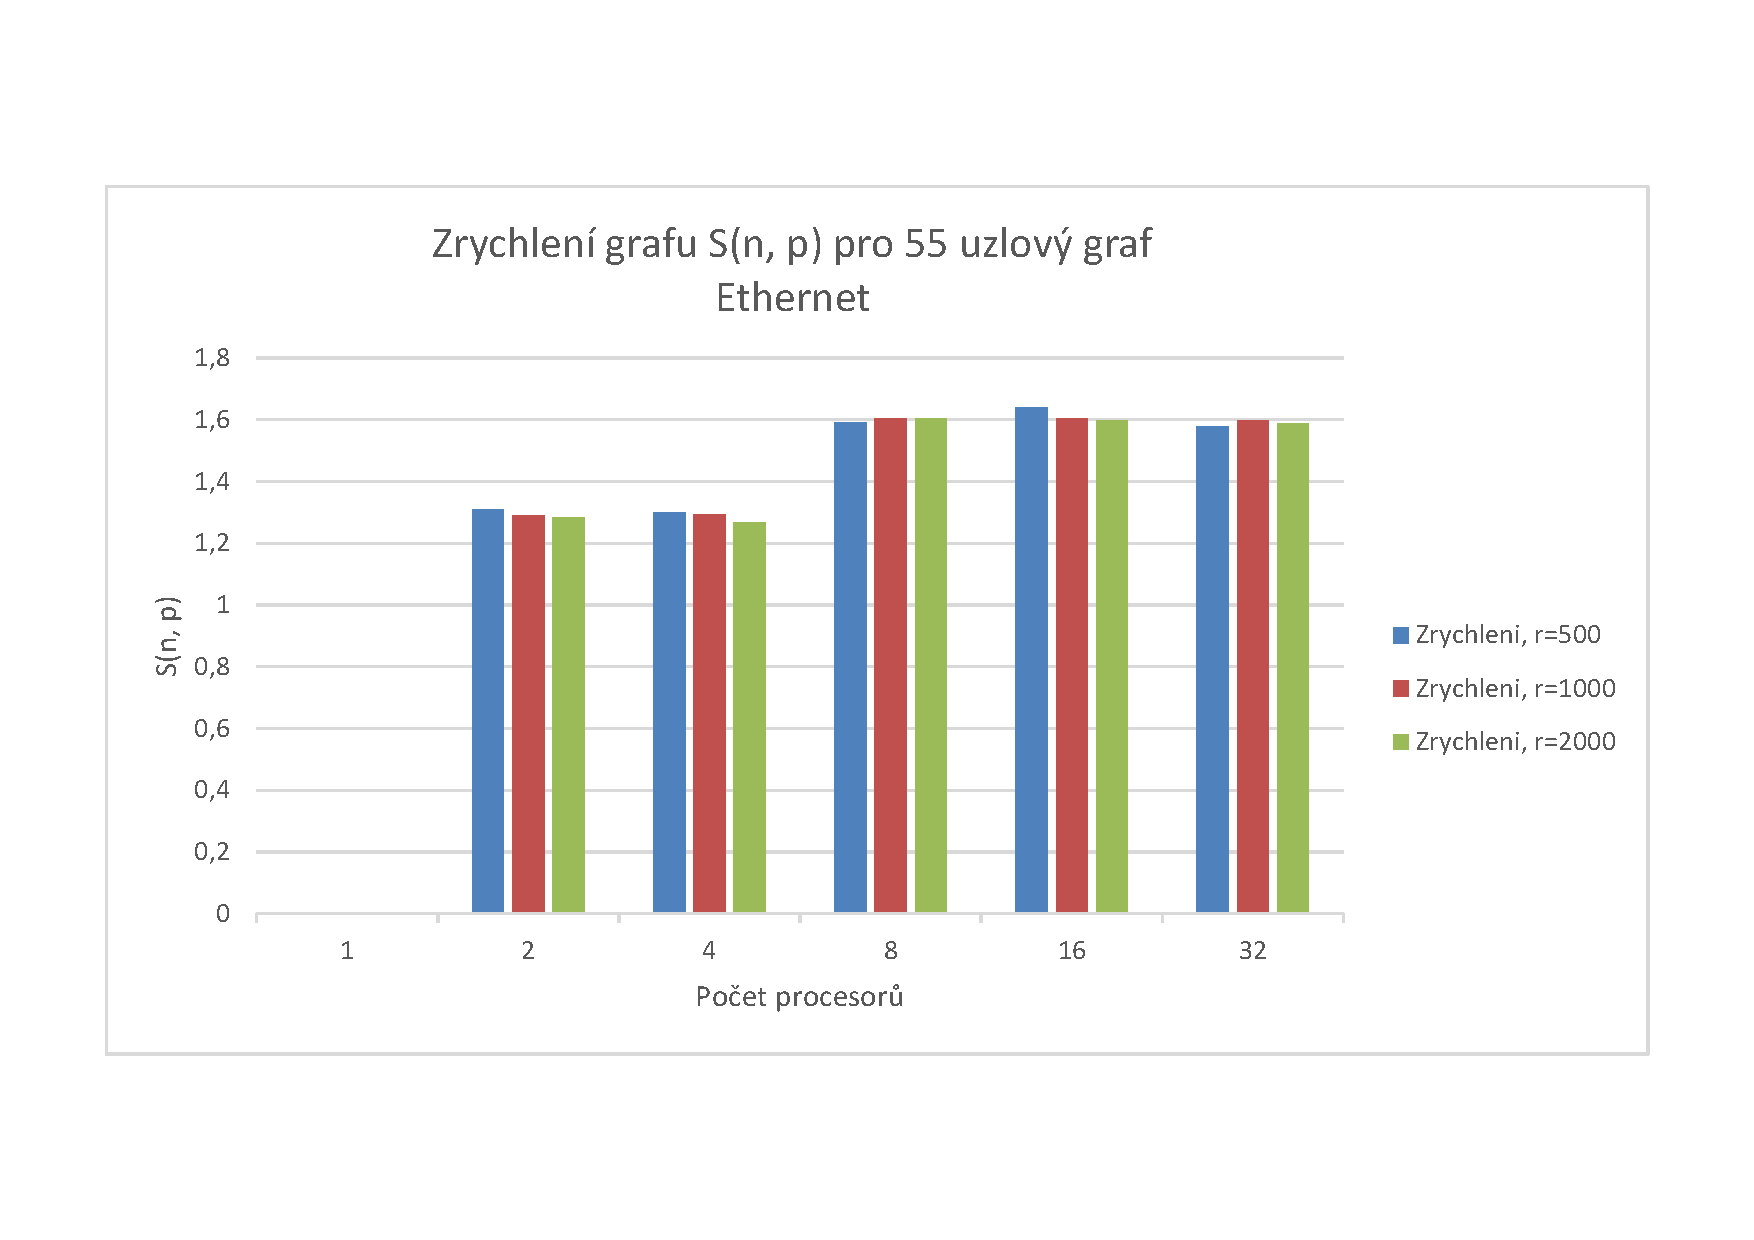
\includegraphics[width=15cm]{zrychleni55.pdf}
\end{figure}

\newpage
\subsubsection{Problém b) 65 uzlový graf}
\begin{table}[h]
	\caption{Naměřené hodnoty pro graf o 65 uzlech}
	\label{tab:namereneHodnotyGraf65}
	\centering
	\begin{tabular}{| c || c | c | c | c | c | c |}
		\hline
		\textbf{Počer procesorů} & \textbf{1} & \textbf{2} & \textbf{4} & \textbf{8} & \textbf{16} & \textbf{32} \\
		\hline \hline
		\textbf{Čas [s], r=500} & 615 & 797 & 727 & 328 & 90 & 95 \\
		\hline
		\textbf{Zrychlení, r=500} & x & 0,77 & 0,85 & 1,88 & 6,83 & 6,47 \\
		\hline
		\textbf{Čas [s], r=1000} & 615 & 1007 & 729 & 331 & 92 & 93 \\
		\hline
		\textbf{Zrychlení, r=1000} & x & 0,61 & 0,84 & 1.86 & 6,68 & 6,61 \\
		\hline
		\textbf{Čas [s], r=2000} & 615 & 794 & 728 & 336 & 92 & 94 \\
		\hline
		\textbf{Zrychlení, r=2000} & x & 0,77 & 0,84 & 1,83 & 6,68 & 6,54 \\
		\hline
	\end{tabular}
\end{table}

\begin{figure}[h]
  \centering
 	\caption{Zrychlení grafu S(n, p) pro 65 uzlový graf - Ethernet}
  	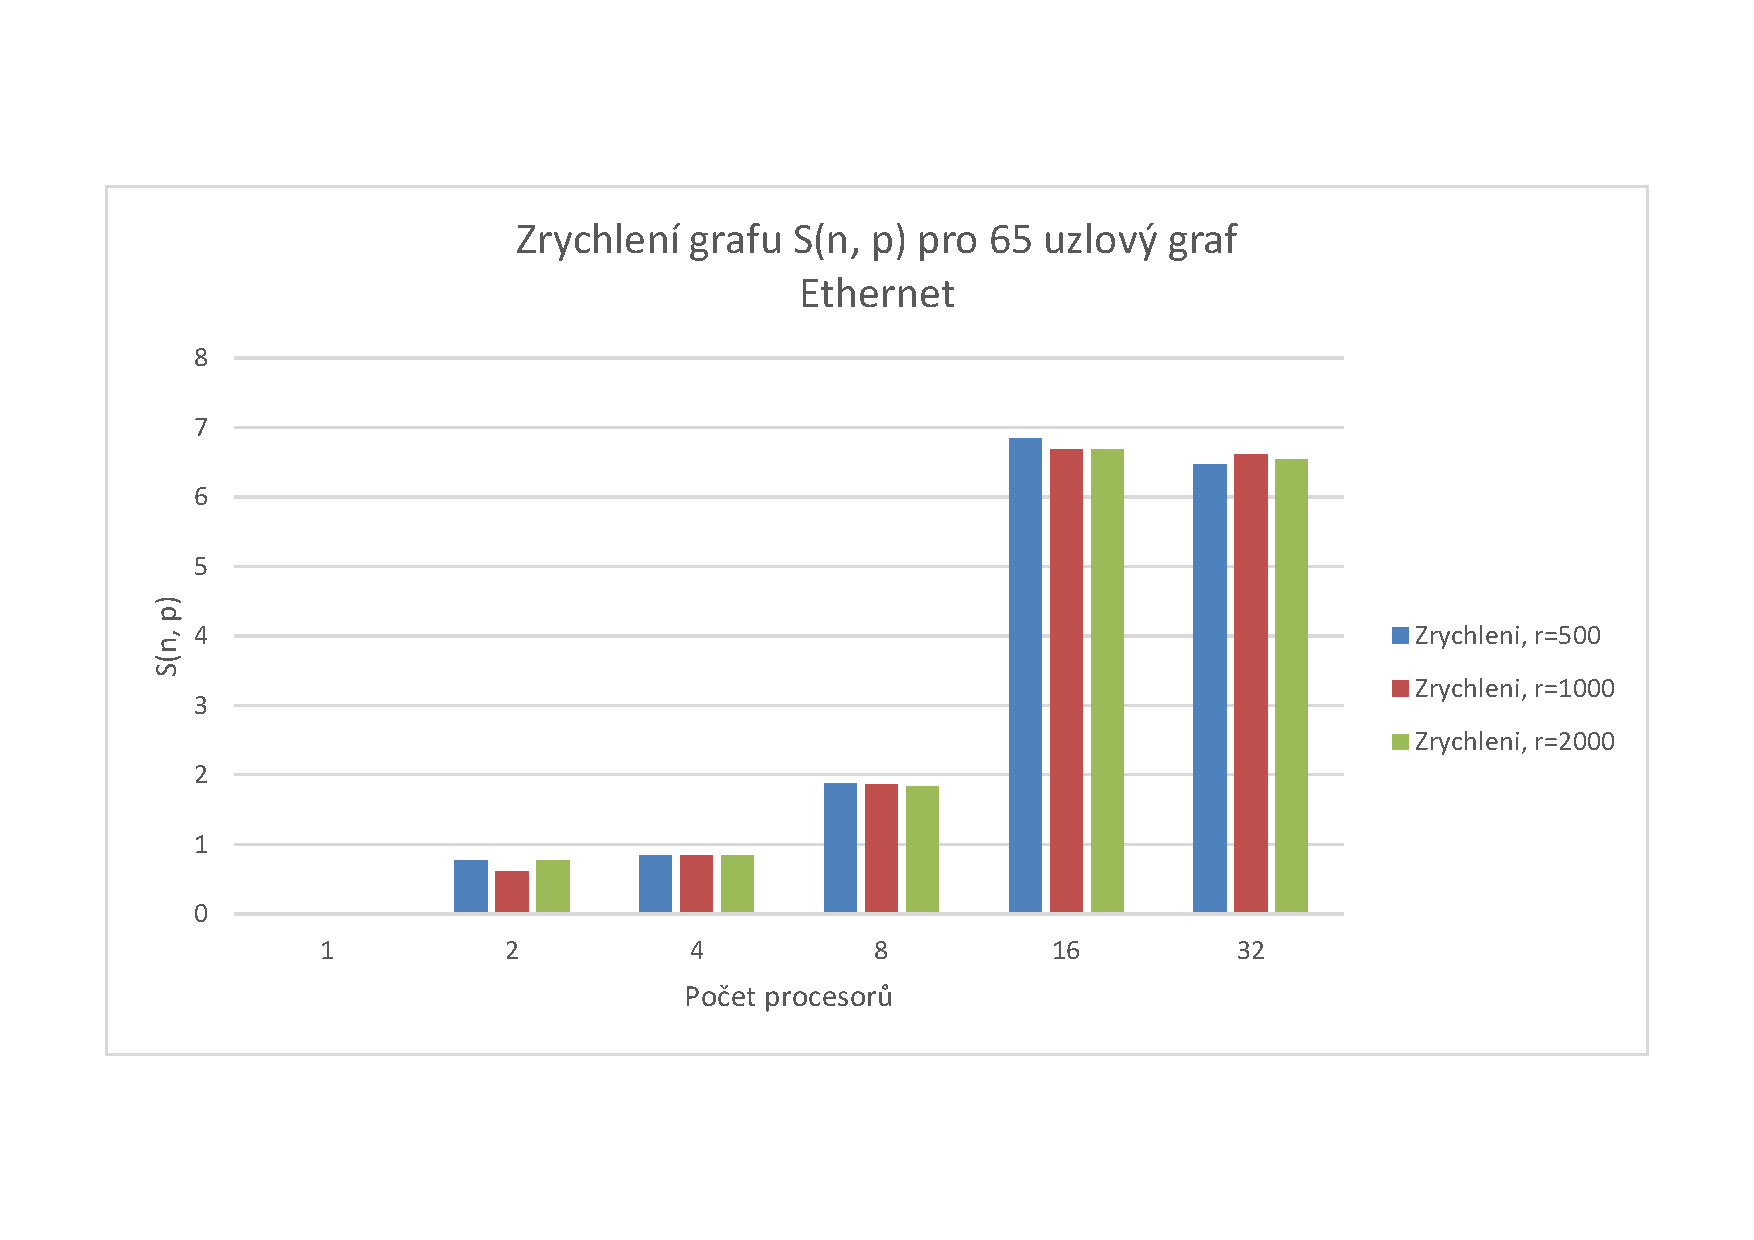
\includegraphics[width=15cm]{zrychleni65.pdf}
\end{figure}

\newpage
\subsubsection{Problém c) 70 uzlový graf}
\begin{table}[h]
	\caption{Naměřené hodnoty pro graf o 70 uzlech}
	\label{tab:namereneHodnotyGraf70}
	\centering
	\begin{tabular}{| c || c | c | c | c | c | c |}
		\hline
		\textbf{Počer procesorů} & \textbf{1} & \textbf{2} & \textbf{4} & \textbf{8} & \textbf{16} & \textbf{32} \\
		\hline \hline
		\textbf{Čas [s], r=500} & 901 & 925 & 704 & 326 & 132 & 134 \\
		\hline
		\textbf{Zrychlení, r=500} & x & 0,97 & 1,28 & 2,76 & 6,83 & 6,72  \\
		\hline
		\textbf{Čas [s], r=1000} & 901 & 924 & 705 & 321 & 133 & 134 \\
		\hline
		\textbf{Zrychlení, r=1000} & x & 0,98 & 1,28 & 2,81 & 6,77 & 6,72 \\
		\hline
		\textbf{Čas [s], r=2000} & 901 & 1191 & 708 & 321 & 132 & 135 \\
		\hline
		\textbf{Zrychlení, r=2000} & x & 0,76 & 1,27 & 2,81 & 6,83 & 6,67 \\
		\hline
	\end{tabular}
\end{table}

\begin{figure}[h]
  \centering
 	\caption{Zrychlení grafu S(n, p) pro 70 uzlový graf - Ethernet}
  	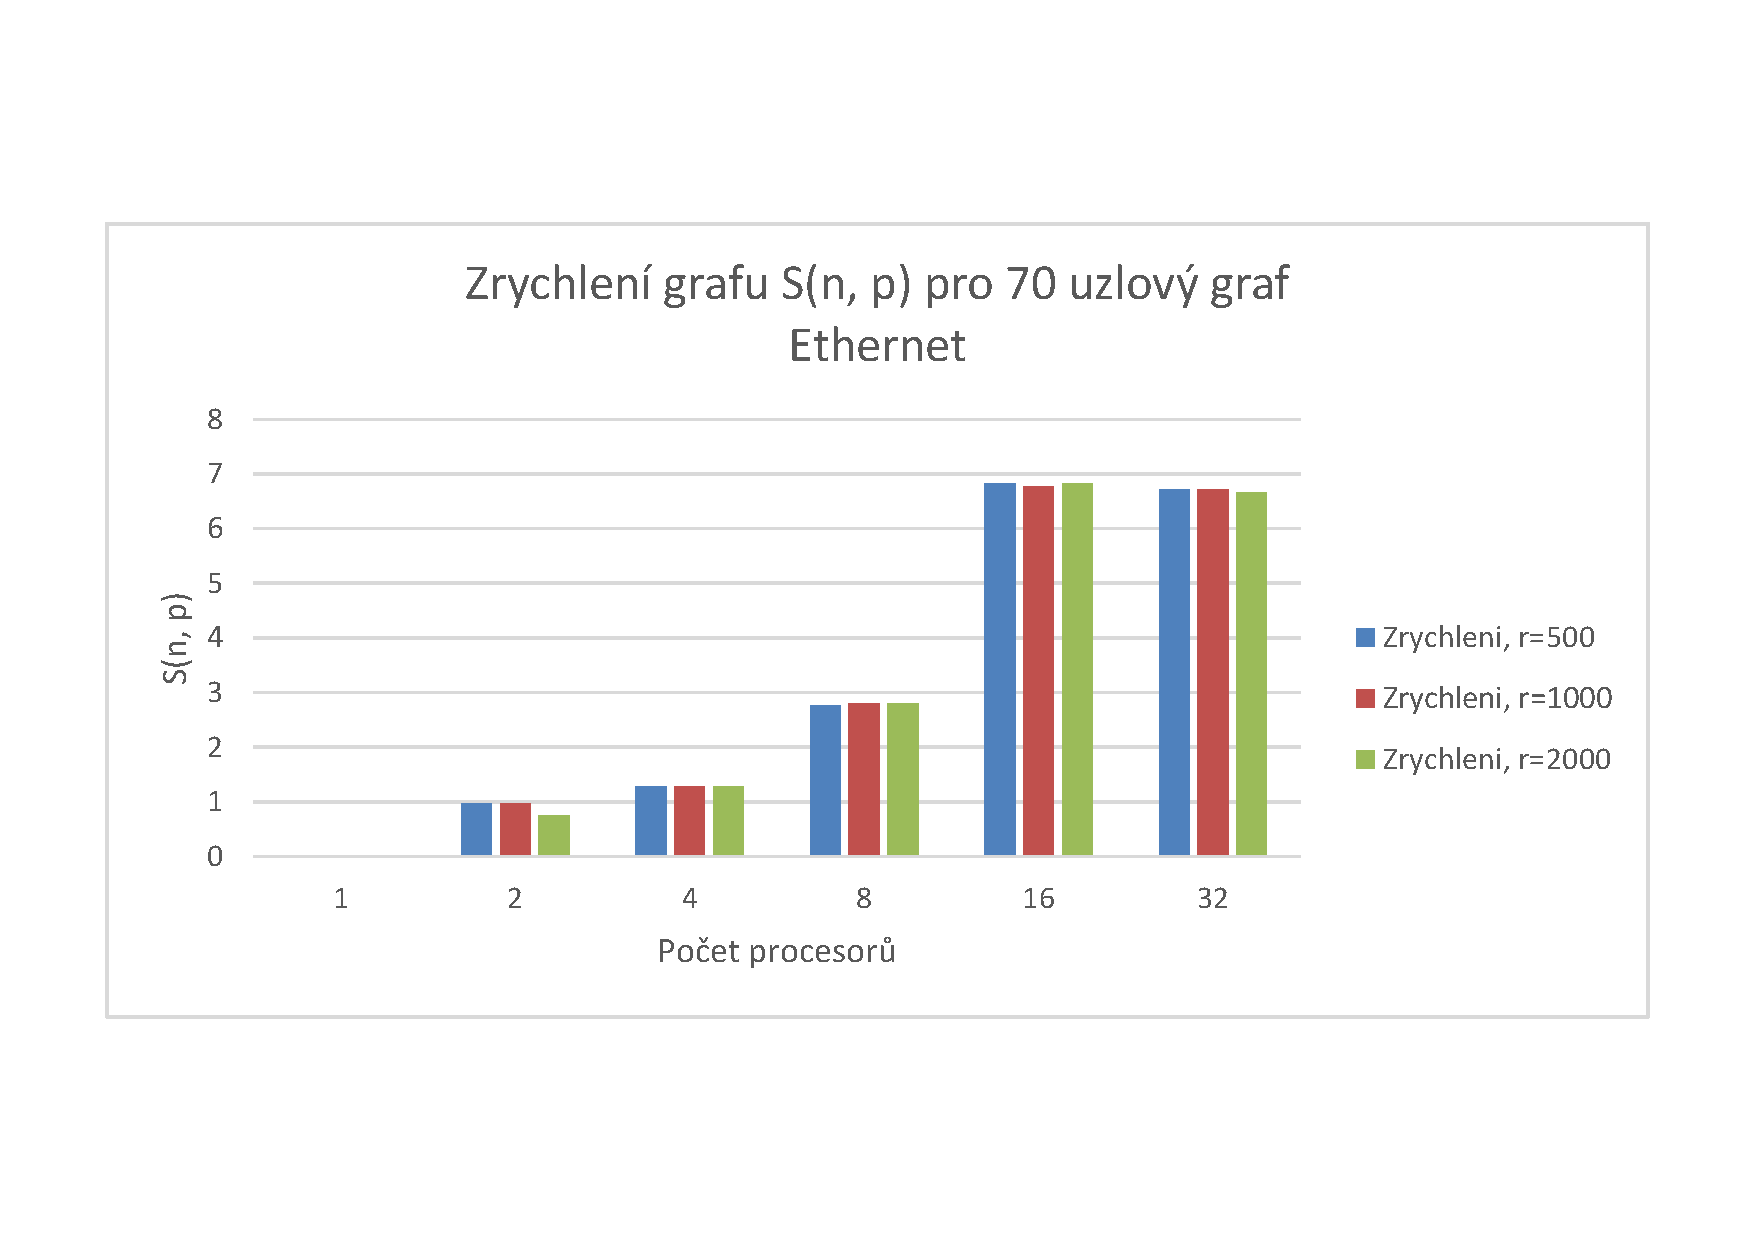
\includegraphics[width=15cm]{zrychleni70.pdf}
\end{figure}

\subsection{Komunikační složitost}
Z naměřených dat jsme vypozorovali, že pro p>16 procesorů začíná být síťová komunikace velká, kde se to odrazilo ve zrychlení paralelního výpočtu. Je to způsobeno nenalezení správné konstanty pro dělení práce pro vysoký počet procesorů, kde pak je komunikace po síti četnější. Pro tuto úlohu jsme nenašli instanci, pro kterou by existovalo superlineární zrychlení. 

\subsection{Granularita}
Granulita pro tuto úlohu nemá cenu dělit více než na 16 procesorů, protože pak už vychází podobné výsledky s malou odchylkou. Je to způsobeno vysokou cenou za síťovou komunikaci a výpočet pro p>16 procesorů začíná být cenově (paralelně) nevýhodný. Výpočty jsou díky lineárnímu zrychlení pořád cenově optimální.\\

Pro malé grafy, které běží na sekvenčním řešení přibližně 5~minut dosahuje stále lineárního zrychlení, ale paralelní cena už je opravdu nízka, kde stojí za zváženou, jestli nechat výpočet běžet na více procesorech.

%%%%%%%%%%%%%%%%%%%%%%%%%%%%%%%%%%%%%%%%%%%%%%%%%%%%%%%%%%%%%%%%5
\section{Závěr}
Implementace sekvenčního algoritmu a následné porovnání naměřených výsledků paralelního algoritmu potvrdilo fakt, že dojde ke zrychlení výpočtu konkrétního problému. 
Paralelní algoritmus by se dal určitě zrychlit při nalezení správné konstanty pro dělení práce pro vysoký počet procesorů, v našem případě p>16, kde by nedocházelo k přílišné komunikaci po síti. V určité vysoké zvolené konstanty by nedocházelo k přerozdělování práce mezi procesory a pak by docházelo ke zpomalení výpočtu.

\appendix


\end{document}